% !TeX root = ../../thesis.tex
\chapter{Bayesian parameter estimation of the computational models}\label{ch:bayesian}

\begin{shaded}
This chapter is based on previously published content in the \textit{Journal of Open Source Education}:\\
M. Barzegari, and L. Geris, ``An open source crash course on parameter estimation of computational models using a Bayesian optimization approach
,'' \textit{Journal of Open Source Education}, vol. 4, p. 89, 2021.\\
This publication included didactical and educational materials in Jupyter Notebooks format to make it possible for readers to follow the principles interactively. The introductory part of the Jupyter Notebook file is included in this chapter as well.
\end{shaded}

\section{Summary}

Parameter estimation is a crucial aspect of computational modeling projects, especially the ones that deal with ordinary differential equations (\gls{ODE}) or partial differential equation (\gls{PDE}) models. Well-known examples in this regard are models derived from a basic balance or conservation law, such as mass balance or heat transfer problems. For real-world applications, these equations contain some coefficients that cannot be obtained directly from published scientific materials or experimental studies \cite{Dehghan2001}. One of the best solutions to this challenge is constructing an inverse problem.

According to \cite{Tarantola1987}, inverse modeling is the use of the results of some measurements of observable parameters to infer the values of the model parameters. Put differently, what we want to do is estimate parameters that cannot be directly measured for our computational model. This is also called parameter estimation or model calibration \cite{Carson2014}. Indeed, we calibrate our model to act similarly to available experimental data, and then this calibrated model can be used to simulate other scenarios that haven't been tested yet in the experiments. This is a common process in a lot of modeling problems in science and engineering.

Take a simple reaction-diffusion equation as an example, in which the change of the concentration of a sample chemical component $C$ is studied over time. By assuming that the correlated chemical reaction is $A + 2B \rightleftharpoons C$, occurring in a diffusible medium (such as a chemical solution), the \gls{PDE} to describe the mass transfer phenomenon over time can be written as \cite{Grindrod1996}:
\begin{equation}
\frac{\partial [C]}{\partial t} = \nabla . \left( D_C \nabla [C] \right) + k_1 [A][B]^2 - k_2 [C]
\end{equation}
in which $[X]$ denotes the concentration of the chemical component $X$, the $D_C$ is the diffusion coefficient of C in the medium, and $k_1$ and $k_2$ are the rates of the forward and backward reactions, respectively. To solve this \gls{PDE} numerically and get quantitative data (the goal of most of the scientific computing projects), we need to know the value of $D_C$, $k_1$, and $k_2$, which is usually hard-to-find in the literature.

As mentioned above, one solution is to to solve the inverse problem, in which we can use optimization techniques to minimize the difference between the model output and experimental data. Bayesian optimization is one of the most efficient approaches in this regard \cite{Mockus1989}. \texttt{HyperOpt} \cite{Bergstra2013} is a Python package that provides easy-to-use interfaces to implement a Bayesian optimization problem, making it a good choice for both educational and practical purposes. In our educational module, we used this package to teach the principles of an efficient parameter estimation pipeline.

For demonstration purposes, an interpolation problem is solved by using the parameter estimation techniques that a computational modeling researcher employs for model calibration. Indeed, the computationally intensive code is replaced with a simple function evaluator, which helps students to learn the core concepts without waiting too much for the process to finish. Students will be guided through several steps of refining the results inside the notebook, where the interactive computing environment of Jupyter facilitates exploring the implementation more efficiently in comparison to traditional educational materials.

\section{Statement of need}

Despite its simplicity, building an inverse problem is hard for many students. The problem is that, although it is relatively simple to describe the process visually, implementing it for a practical application becomes challenging in its early stages. In this educational module, a simple optimization problem is implemented in a Jupyter notebook to teach students how to construct an inverse problem and tune it to get better results in such a problem. In this way, students can work on a real-world optimization problem in an interactive environment and learn the concepts behind taking advantage of a modern optimization method (Bayesian approach) for parameter estimation of a computational model.

Our notebook is a modern learning module for relatively old and frequently-used concepts (global optimization, Bayesian techniques, inverse problems). It has been designed to be useful for both teachers and students. Students can use it as a self-study guide for parameter estimation and inverse problem construction, while teachers can change the underlying problem to any other desired one easily and make the learning module compatible with their own teaching requirements.

\section{Learning objectives}

Upon completion, students will be able to:

\begin{itemize}
\item
Understand the concept and necessity of parameter estimation in science and engineering
\item
Describe what the whole process of Bayesian optimization is all about
\item
Define and implement a Bayesian optimization workflow for parameter estimation of common use-cases
\item
Critically evaluate the output of the process and fine-tune the setup of the Bayesian optimization
\item
Apply the obtained knowledge to any kind of models that are commonly used in science and engineering
\end{itemize}

\section{Prerequisites}

In order to go through the learning module, the students should have a working knowledge of programming in Python. Additionally, a basic understanding of mathematics is required to get the concept of models in science and engineering. The given example is a mathematical model derived from differential equations, so knowledge of differential equations can help to understand the importance of parameter estimation in these widely-used models. However, in case of necessity, the example can be replaced by any other relevant one for the target learners.

\section{Pedagogy and instructional design}

The provided material is in the format of a crash course, which is suitable for being taught in one session of undergraduate or graduate courses for science and engineering students. Courses to which this material is relevant can be
``optimization'', ``scientific computing'', or ``parametric design''. The material may also be useful for relevant educational projects for the target students, in which they can employ the learned techniques to construct efficient inverse problems for parameter estimation.

The teaching strategy is based on the worked-example effect \cite{Chen2015}, in which an example of parameter estimation is fully implemented to allow students to play with and modify the code to have their own reflection in class discussions. Basic prior knowledge of Python suffices as the problem doesn't involve students with complicated programming stuff. The student-centric characteristic of this crash course helps teachers to adopt the material easily and integrate it into an existing syllabus of relevant courses in science and engineering.

\section{Getting started}

The learning material is provided as a single Jupyter notebook, in which all the steps of constructing an inverse problem are described in detail with accompanying Python codes. A very simple simulation code (in the context of an interpolation problem) is also provided and can be found in the repository. The code inside the notebook calls this external program at certain points to mimic the interaction of the parameter estimation routine and the main computational code that contains the unknown parameters.

To get started with the module, the user should set up the environment first. The setup instructions are provided in the \texttt{README.md} file of the repository. After setting up the Jupyter notebook and installing the required packages, the user can navigate to the \texttt{src} folder and run the notebook file. No further action is needed as the content of the notebook is self-explanatory and easy-to-follow.

\section{Acknowledgements}

This research is financially supported by the Prosperos project, funded by the Interreg VA Flanders – The Netherlands program, CCI grant no. 2014TC16RFCB046 and by the Fund for Scientific Research Flanders (FWO), grant G085018N. We acknowledge support from the European Research Council under the European Union's Horizon 2020 research and innovation programmen, ERC CoG 772418.


\begin{subappendices}

\section{A glimpse of the Jupyter notebook}

\subsection{Introduction}

As the name implies, the parameter estimation process deals with approximating unknown parameters, the factors that define a system or its operation. In science and engineering, this can be seen as a sub-category of optimization techniques since we seek to find the optimal state of a system. After finding the desired state, we look for the parameters contributing to such a state. It is indeed what parameter estimation is all about. Seems complex? Look at it as a calibration process, in which a machine, tool, or system is tuned to produce a correct output. Imagine you want to calibrate a machine with 3 knobs. How do you do the calibration?  You compare the output with a reference, something you know the machine should produce, and then try to adjust the knobs such that the output matches the reference. It is how calibration works, no? Take a thermometer as an example. You have a reference temperature, like boiling water at 100 degrees Celsius, and 3 knobs on the device. You continue turning the knobs to see 100 appearing on the machine, and by doing that, you calibrate the thermometer. In this way, you have estimated the unknown parameters (the 3 knobs) of the device. After being calibrated,  you can use the thermometer to measure any temperature.

Now, instead of the machine, assume you want to perform the same process on an engineering system. Each system (or, let's say, model) has a certain number of parameters to be tuned. After calibrating the system (model) with the reference data (a data we already know is correct), we can assure that the system's output is more or less valid if being used for another measurement (prediction). Real-world systems in science and engineering contain some parameters that cannot be obtained directly from published scientific materials or experimental studies. Thus, we should estimate them using a calibration (optimization) strategy, a process that is generally called an inverse problem.

An inverse problem in science is usually referred to the process of calculating the causal factors from a set of observations that have produced them. Inverse problems are important because they tell us about parameters that we cannot directly observe. That's exactly what we want to do: estimating parameters that we cannot directly measure for our model. Indeed, we calibrate our model to act similarly to available experimental data, and then this calibrated model can be used to simulate other scenarios that we have not tested in experiments. This concept is similar to the training process of machine learning models. You train the model by making it fit to previously available data and asking it to predict unseen data.

To construct an inverse problem for computational models, we can take advantage of conventional optimization approaches. The goal is to minimize or maximize a function, or more technically speaking, an objective function. Mathematical optimization is selecting the best element (concerning some criterion) from some set of available alternatives.  In the simplest case, an optimization problem consists of maximizing or minimizing an objective function by systematically choosing input values from an allowed set and computing the output of the system. More generally, optimization is the process of finding the optimum value of an objective function given a defined domain (or input). To wrap up, the essential concepts here are the objective function (what we want to minimize) and the domain space (values of the parameters over which we minimize the objective).

Back to our example problem, our objective function will be the difference between the produced output of our simulation and the experimental data of the exact condition, which is also called "loss". In other words, we change the coefficients such that the simulation output would be the same as (or close to) the experimental data that we already have. To this end, we can choose random values out of the domain space (the range that we search for appropriate values), evaluate the model with those values, and continue this process till we find the lowest loss possible. This can be a good approach as long as the cost function evaluation is cheap, which means the simulations run fast (because we need to run the simulation to evaluate the cost function). The problem is, for most of the real-world models, running each simulation takes quite long. As a result, each iteration of the optimization algorithm is not cheap anymore. To overcome this issue, we use a Bayesian optimization strategy, a method that is usually employed to optimize expensive-to-evaluate functions.

\subsection{Bayesian optimization}

To describe how the Bayesian optimization approach helps us to overcome the problem mentioned above, I use the great description made by @WillKoehrsen\footnote{\url{https://github.com/WillKoehrsen}}. I cannot explain it better (you can find the full interactive document at\\ \url{https://github.com/WillKoehrsen/hyperparameter-optimization}:

\begin{itshape}
Evaluating the objective function is the expensive part of optimization, so ideally, we want to limit calls to this function. One way we can limit calls is by choosing the next values to try in the objective function based on the past results. Bayesian optimization differs from random or grid search by doing exactly this: rather than just selecting from a grid uninformed by past objective function evaluations, Bayesian methods take into account the previous results to try more promising values. They work by constructing a probability model of the objective function (called a surrogate function) $p(\text{score} | \text{parameters})$ which is much easier to optimize than the actual objective function. $p (A\mid B)$, the conditional probability, is the probability of A given B, i.e., A after B is observed.

\newglossaryentry{SMBO}{name={SMBO},description={sequential model-based optimization}}

After each evaluation of the objective function, the algorithm updates the probability model (usually given as $p(y | x)$ incorporating the new results. Sequential Model-Based Optimization (\gls{SMBO}) methods are a formalization of Bayesian optimization that updates the probability model sequentially: every evaluation of the objective function with a set of values updates the model with the idea that eventually the model will come to represent the true objective function. This is an application of Bayesian Reasoning. The algorithm forms an initial idea of the objective function and updates it with each new piece of evidence.

The next values to try in the objective function are selected by the algorithm optimizing the probability model (surrogate function), usually with a criterion known as Expected Improvement. Finding the values that will yield the greatest expected improvement in the surrogate function is much cheaper than evaluating the objective function itself. By choosing the next values based on a model rather than randomly, we hope that the algorithm would converge to the true best values much quicker. The overall goal is to evaluate the objective function fewer times by spending a little more time choosing the next values. Overall, Bayesian Optimization and \gls{SMBO} methods:

\begin{itemize}
\item
Converge to a lower score of the objective function than random search
\item
Require far less time to find the optimum of the objective function
\end{itemize}

So, we get both a faster optimization and a better result. These are both two desirable outcomes, especially when we are working with heavy computational models!
\end{itshape}

According to this simplified description, Bayesian optimization is a great candidate to perform the parameter estimation of \gls{PDE}-based computational models. If you are interested to know more about the mathematical aspects of the Bayesian optimization, you may have a look at the SigOpt Bayesian Optimization Primer.

\newglossaryentry{TPE}{name={TPE},description={tree-structured Parzen estimator}}

In this notebook, we implement the whole process of a Bayesian optimization strategy, including constructing a cost function by calling the simulation code, performing the optimization, and postprocessing the results. To do this, we use Python and HyperOpt, an open-source Python library for Bayesian optimization that implements \gls{SMBO} using the Tree-structured Parzen Estimator (\gls{TPE}). \gls{TPE}, along with Gaussian Processes and Random Forest Regression, are the algorithms that can be used in the \gls{SMBO} method to construct the probability model (surrogate function). We don't need to worry about implementing the algorithm because Hyperopt takes care of that for us. We have to make sure we have correctly defined the objective function and the domain of values to search over.

\subsection{Sample problem}

Instead of a \gls{PDE} model, we use a more straightforward problem to focus more on the optimization rather than the numerical simulation of the \gls{PDE}. The problem with which the optimization algorithm interact is fitting a 4th-order polynomial equation on some experimental data. You should notice that the optimization algorithm is entirely unaware of the fitting problem behind the objective function.

The objective function is implemented in a general way: calling the external simulation code, gathering produced output, and computing the loss. To make this as real-world as possible, I implemented an external Python code that takes polynomial coefficients and computes the function values on desired points. This data is saved on the disk and then retrieved by the objective function of the main optimization code to calculate the loss. In a real-world application, the external simulation code takes the coefficients (such as the reaction rates in the above \gls{PDE} example), performs the simulation, and writes the output to the disk. The rest of the process is the same. In the next step, the optimization algorithm changes the parameters and calls the external simulation code again to see the loss of the new parameters. This process continues iteratively to a certain number of iterations.

The experimental data, which are indeed 21 points of a 4th-order polynomial function in the range $[0, 5]$, are stored in a CSV file. Each line contains one point, better to say a pair of two values defining a point, and this exactly what it can be in a real scenario. For example, it can contain the value of a chemical component concentration over time, in which the first and second values of each line would be time and concentration, respectively.

The optimization output of this sample problem will be similar to Fig. \ref{fig:bayes_output}.

\begin{figure}[h]
\centering
\medskip
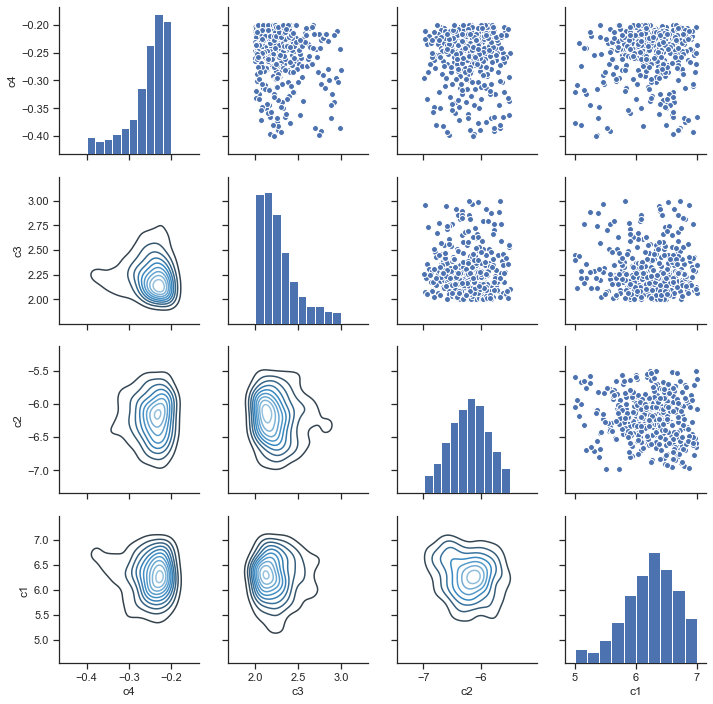
\includegraphics[width=\textwidth]{pair_grid.png}
\caption[A typical output of the parameter estimation process]{A typical output of the parameter estimation process, plotted using the Seaborn Python package, which shows how the optimization algorithm has chosen the values of different parameters in different iterations by comparing the distribution of points 2 by 2 for 4 unknown parameters of the polynomial model.} \label{fig:bayes_output}
\end{figure}

\end{subappendices}

%%%%%%%%%%%%%%%%%%%%%%%%%%%%%%%%%%%%%%%%%%%%%%%%%%
% Keep the following \cleardoublepage at the end of this file,
% otherwise \includeonly includes empty pages.
\cleardoublepage
